\section{科研应用与代表性系统}
\subsection{文献综合与研究问题形成}
文献工作既是科研智能体较易进入的场景，也是后续研究的知识基础。
PaperQA2将搜索、文献处理、证据整理与带引用的回答联系起来，并针对检索、综合及矛盾识别设计评价\cite{paperqa}。
相较于仅在给定段落上问答，这类系统需要决定继续搜索何种材料，以及何时已有证据足以回答问题。
研究中的矛盾识别结果还说明，资料综合不仅涉及归纳共识，也涉及寻找不能被同时接受的表述。
这些任务使评价从答案流畅性转向材料覆盖与来源支持，具有直接的科研实用价值。

ResearchAgent以核心论文为起点，结合学术关系和概念知识生成问题、方法与实验构想，
再通过评审代理的反馈迭代修订\cite{researchagent}。
SciAgents进一步将本体知识图谱、语言模型与多主体讨论结合，用于探索材料相关概念之间的联系\cite{sciagents}。
二者分别强调围绕论文展开的构思和图结构支持的跨概念关联。
这类方法为从已有知识中发现研究切入点提供了可操作途径，也使图组织的价值从信息检索延伸到候选生成。

不过，构思质量仍有多个层次。
新颖性关注与已有工作的差别，合理性关注机制或方法是否自洽，可检验性则要求提出可以实施的区分手段。
人工或模型评价可以检验候选是否值得进一步研究，但不能代替候选真正实施后的证据。
因此，文献与假设系统最适合被理解为研究准备和探索工具，其产出需要在实验设计阶段继续筛选。
这一定位能够保留系统的创造性价值，也避免把构思评分直接解释为发现成功。

\subsection{计算实验与端到端研究}
计算科研具有数据、程序和指标可被统一工具链处理的特点，是端到端研究的重要试验场。
The AI Scientist早期系统将创意生成、代码修改、运行、分析、写作与模拟评审连接起来\cite{scientist}。
其预设模板限定了初始研究空间，但也降低了环境配置与基础实现的不确定性，便于集中考察想法生成和实验迭代。
第二版系统减少对人工代码模板的依赖，使用实验树搜索扩展候选，并引入视觉语言反馈改善图表与呈现\cite{scientistv2}。
从固定模板到搜索式实验管理，反映了自动科研由局部修改向更开放实现空间的发展。

2026年的期刊报告同时研究聚焦模式与开放模式，并进一步讨论自动评审及实际工作坊评审\cite{scientistjournal}。
这比仅由系统内部评价生成论文提供了更多外部参照。
但工作坊个案的评价范围、主题设置和接受条件仍需与通常意义上的广泛科学贡献区分。
早期系统、第二版与期刊报告属于同一研究脉络，不能作为三次独立的全面能力验证累加。

Agent Laboratory采用不同的协作定位：从人提供的研究想法出发，组织文献、实验与报告，
并允许在各阶段引入人的反馈\cite{lab}。
其价值在于把自动化目标与研究者的已有目标相结合，而不要求系统独立决定所有问题。
原文同时比较模型后端、人工评价和不同参与方式，报告了特定设置中自动总体评分6.1/10与人工3.8/10的差异。
这一结果表明，研究报告的可读性、实验质量和评审模型偏好需要分开评价。
对于协作式工具，实际帮助可能体现为降低实现负担，也可能体现为研究者更容易发现计划中的问题，
因而仅用最终论文评分还不能完整衡量其效用。

\subsection{假设搜索与跨学科研究协作}
AI co-scientist围绕专家给定的目标，组织生成、反思、排序、演化等功能代理，
通过候选比较与迭代形成研究建议\cite{cosci}。
这种设计将计算资源用于扩大和修订假设空间，与按既定方案执行一次实验不同。
其排序反馈有助于筛选候选，但排名反映的是比较标准下的相对优势，不能直接解释为命题成立的概率。

该研究在药物再利用、肝纤维化靶点及细菌基因转移机制等方向报告验证案例\cite{cosci}。
各案例的证据性质不同：细胞或类器官结果提供特定实验体系中的支持，
与尚未公开的实验机制相符合，则体现另一种知识推断能力。
这些案例说明候选生成可以与真实科研检验衔接，但其一般化范围仍取决于问题选择和后续实验。

Virtual Lab以负责人代理和专业代理组成研究会议，由人类提供高层反馈，
将蛋白质语言模型、结构预测和分子能量评价整合到纳米抗体设计流程\cite{virtual}。
论文选择92个候选进行实验表征，既呈现了有前景的候选，也显示计算指标与实际功能的差异。
其中78个候选具有更高的相应结构置信度指标，60个具有更优的Rosetta结合能，
但不同亲本系列的实际结合表现并不一致。
这说明专用计算模型、代理组织和实验验证承担不同作用，不能仅凭代理参与就把所有收益归为LLM推理。
对跨学科研究而言，多代理更有意义的贡献是组织已有专长和工具，并使不同研究环节形成可追踪联系。

\subsection{专业工具与实体实验}
ChemCrow将18种专业工具与语言模型结合，用于化学相关问题、合成规划及实验任务\cite{chemcrow}。
专门工具补充了基础模型难以可靠完成的化学计算、检索和执行能力。
这一设计体现了通用代理与领域工具之间的分工：模型负责解释目标和选择步骤，工具负责具有明确输入输出的专业操作。
工具覆盖范围、输入表达和输出解释因而与模型能力同样重要。

Coscientist进一步将网络检索、装置文档、代码执行和实验设备整合，展示化学实验从自然语言要求到执行与产物检查的过程\cite{chem}。
图\ref{fig:physical}左侧概括其关键步骤，右侧保留原论文的实验谱图。
在这一流程中，装置文档能够帮助修正调用方式，色谱与质谱则提供区别于语言评价的产物证据。
研究因此不只依赖系统是否声称完成任务，还可以检查实验输出与参照物之间的关系。

\begin{figure*}[t]\centering
\begin{minipage}[c]{.49\textwidth}\centering
\begin{tikzpicture}[node distance=4mm,b/.style={draw=ZJUIBlue,rounded corners=1.5pt,text width=62mm,minimum height=9mm,align=center,font=\small},a/.style={-{Stealth[length=2mm]},thick,draw=ZJUIBlue}]
\node[font=\bfseries\small] (title) {从任务指令到可检查的实验输出};
\node[b,below=3mm of title] (r) {查阅文献与装置文档};
\node[b,below=of r] (p) {选择方案并生成执行程序};
\node[b,below=of p] (e) {调用液体处理与分析设备};
\node[b,below=of e] (v) {将产物测量与参照数据比较};
\draw[a](r)--(p);\draw[a](p)--(e);\draw[a](e)--(v);
\draw[a,draw=EvidenceGreen](e.east) to[out=0,in=0] (p.east);
\node[below=3mm of v,font=\footnotesize,align=center,text width=66mm] {装置反馈修正操作；测量结果支持实验判断。};
\end{tikzpicture}
\end{minipage}\hfill
\begin{minipage}[c]{.235\textwidth}\centering
{\small Suzuki反应}\par\vspace{2mm}
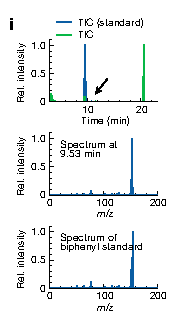
\includegraphics[width=\linewidth]{figures/coscientist-suzuki.pdf}
\end{minipage}\hfill
\begin{minipage}[c]{.235\textwidth}\centering
{\small Sonogashira反应}\par\vspace{2mm}
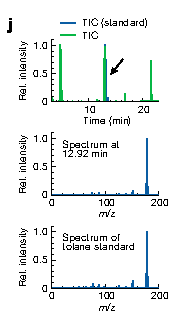
\includegraphics[width=\linewidth]{figures/coscientist-sonogashira.pdf}
\end{minipage}
\caption{科研代理与实体实验验证的衔接。左部依据Coscientist流程归纳\cite{chem}；
右部摘自Boiko等原图5i、5j，分别包含色谱及对应质谱与标准参照。图中曲线、坐标与数值保持原样，仅提取面板并调整排列。
原图版权为作者，依据\href{https://creativecommons.org/licenses/by/4.0/}{CC BY 4.0}转载；数据不是本文实验结果。}
\label{fig:physical}\end{figure*}

实体反馈提高了某些判断的可检查性，也使资源与操作约束更加突出。
Coscientist的部分物理操作仍由人工完成，可探索的试剂和设备范围也由实验设置限定\cite{chem}。
因此，系统应在明确资源边界内评价，不宜把特定装置上的成功直接扩展为开放实验室中的普遍自主能力。
与纯计算场景相比，实体系统更需要在计划阶段考虑操作权限、异常中止、测量噪声和验证成本。

\subsection{不同科研路径的比较}
表\ref{tab:systems}从研究对象与反馈方式总结代表系统。
文献与构思系统的主要产物是证据综合和候选问题，计算系统便于反复执行，实体系统则可以获得更直接的经验观察。
不同路线的自动化覆盖与验证深度相互独立：覆盖更多阶段可以减少人工交接，但也增加错误跨阶段传播的机会；
加入实验测量能够检验具体命题，却仍然依赖有效的对照与解释。
因此，更有意义的比较不是给系统排列统一自主等级，而是说明它们在哪些条件下推进了哪些研究活动。

\begin{table*}[t]\centering\tabletext
\caption{代表性科研系统的主要组织方式与证据来源。不同报告之间的任务、模型、工具和人工参与不同，不作统一成绩比较。}
\label{tab:systems}
\begin{tabularx}{\textwidth}{@{}>{\raggedright\arraybackslash}p{29mm}YYY@{}}\toprule
系统 & 研究对象与组织重点 & 反馈或验证方式 & 主要解释边界\\\midrule
PaperQA2\cite{paperqa} & 文献检索、综合与矛盾识别 & 文献任务基准及专家比较 & 文献综合能力不等同于实验发现能力\\
ResearchAgent / SciAgents\cite{researchagent,sciagents} & 论文关系、概念图谱与迭代构思 & 评审反馈、人工或模型评价与案例 & 候选质量仍需后续实施和检验\\
The AI Scientist系列\cite{scientist,scientistv2,scientistjournal} & 模板研究、实验搜索与论文生成 & 程序实验、自动评审及工作坊案例 & 同一研究系列；个案评审有其适用范围\\
Agent Laboratory\cite{lab} & 人给定想法上的研究协作 & 人工评价、后端与参与方式比较 & 人工帮助及评价差异需单独报告\\
AI co-scientist\cite{cosci} & 多候选生成、比较和演化 & 专家反馈与部分生物医学实验 & 排序不是命题真值，验证类型存在差异\\
Virtual Lab\cite{virtual} & 跨学科会议与专用计算工具整合 & 纳米抗体设计后的实验表征 & 计算指标、表达与功能为不同评价目标\\
ChemCrow / Coscientist\cite{chemcrow,chem} & 专业工具调用与实体执行 & 专家检查、仪器观察及产物分析 & 工具覆盖、装置条件和人工操作限制范围\\\bottomrule
\end{tabularx}\end{table*}
